% Template for FMI-2011 paper; to be used with:
%          fmiconf.sty - LaTeX style file, and
%          IEEEbib.bst - IEEE bibliography style file.
% --------------------------------------------------------------------------
\documentclass{article}
\usepackage{fmiconf,amsmath,epsfig,graphics}
%Change babel Language for different LaTeX "Fixed Names"
\usepackage[ngerman]{babel}
\usepackage[hyphens]{url}
\usepackage{hyperref}
\usepackage[utf8]{inputenc}
\usepackage{enumitem}
\setlist[itemize,1]{leftmargin=15pt,rightmargin=15pt}

% Place images in the folder images
\graphicspath{{images/}}

% Example definitions.
% --------------------
%\def\x{{\mathbf x}}    
%\def\L{{\cal L}}

\title{Einsatz von Mobile Devices mit Freihand-Gestenerkennung als Präsentationsplattform im professionellen Umfeld}

\name{Thomas Rehm, Saskia Schreiber}

\address{Technische Hochschule Mittelhessen\\Friedberg, Hessen}

\begin{document}
%\ninept
\maketitle

\begin{abstract}
In dieser Arbeit wird untersucht, ob sich die bisher gängige Ausrüstung für Präsentationen im Arbeitsumfeld, bestehend aus Laptop, Fernbedienung/Maus, Kabelverbindung und Beamer, durch flexiblere Hardware und Software ersetzen und dadurch vereinfachen lässt. Der Zielaufbau ist ein Mobilgerät mit Gestenerkennung als Eingabemedium sowie eine kabellose Verbindung zum Ausgabegerät, wodurch sich die benötigten Komponenten erheblich reduzieren und die Bedienung intuitiver wird. Um dies auf Softwareseite zu ermöglichen, kommt eine Android-App in Kombination mit Webtechnologien zur Realisierung der Gestenerkennung zum Einsatz, die von den Autoren prototypisch entwickelt wurde. Auf Hardwareseite wird der aktuelle Stand kabelloser Übertragungsprotokolle für Screen Mirroring geprüft und es werden Lösungsansätze für ältere Infrastruktur vorgestellt. 
\end{abstract}

\begin{keywords}
mobiles Endgerät, Freihandgesten, Gestensteuerung, Präsentation, Screen Mirroring, SmartTV
\end{keywords}

\section{Einführung}
Seit der Ablösung des Overhead-Projektors durch Laptop und Beamer kamen viele Dienste und Technologien auf den Markt, um das Erstellen von Präsentationen zu vereinfachen. 
Die eingesetzte Hardware hat sich dagegen nicht wesentlich verändert: Immer noch sind Laptop und Maus (oder separate Fernbedienung) in der Regel fester Bestandteil der Ausrüstung. \\
Durch die steigende Nutzung und Verbreitung von mobilen Endgeräten sowie vernetzten Ausgabe-Geräten (Beamer/SmartTV) stellt sich jedoch die Frage, ob man daraus nicht ein einfacheres Setup schaffen kann. Einfacher durch reduzierte Infrastruktur: Mobilgerät statt Laptop, kabellose Verbindungen statt direkter Verkabelung; einfacher aber auch mit dem Wegfall separater Steuerungsgeräte durch intuitive Gestensteuerung. \\
Somit ist diese Arbeit keine Vorstellung einer neuen Technologie. Sie untersucht stattdessen, ob sich mittlerweile etablierte Technologien zu einem neuartigen Konstrukt verbinden lassen, das die Nachfolge klassischer Präsentations-Setups antreten kann.

\begin{figure}[htb]
\begin{minipage}[b]{1.0\linewidth}
  \centering
\centerline{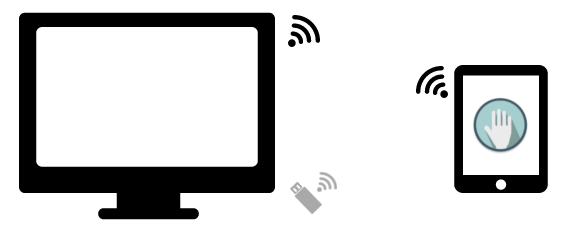
\includegraphics[width=1\linewidth]{aufbau.jpg}}
\end{minipage}
\caption{Illustration des vereinfachten Setups: SmartTV links, Mobilgerät mit Gesture Control rechts. Verbindung entweder direkt oder mit optionalem TV-Stick (grau).}
\label{fig:setup}
\end{figure}


\section{Stand der Technik}
\subsection{Stationäre Geräte zur Gestensteuerung}
Die Nutzung von Freihandgesten als Eingabemedium ist an sich kein neues Konzept.\\
Ein sehr prominentes Beispiel dafür ist die Steuerungshardware Kinect, mit der sich Windows-Geräte und die Spielekonsole Xbox 360 komplett ohne Controller bedienen lassen. Dank eines umfangreichen SDKs können Entwickler mit der Kinect nicht nur Spiele steuern, sondern die unterschiedlichsten Applikationen mit Körperbewegungen in Verbindung bringen. Da der Benutzer in der Regel frontal vor dem Gerät steht, lassen sich Bewegungen des ganzen Körpers nachverfolgen.\\ 
Die Kinect fällt in die Kategorie der stationären Systeme, die alle dank ordentlicher Rechenleistung eine große Genauigkeit bei der Interpretation von Bewegungen erlauben. Für die Steuerung von Präsentationen, wo im Prinzip nur links-rechts-Bewegungen der Hand eine Rolle spielen, wird dies gar nicht benötigt. Dafür fällt der Nachteil der stationären Geräte stark ins Gewicht: Sie sind für den spontanen Einsatz außer Haus zu unflexibel, der Transport und Aufbau zu kompliziert für den fachfremden Präsentierenden.
\subsection{Gestensteuerung auf Mobilgeräten: Samsung Gesture SDK}
Gestensteuerung auf Mobilgeräten wiederum hat andere Voraussetzungen und daher auch andere Ziele. Die Genauigkeit ist durch geringere Prozessorleistungen limitiert, die Aufnahmemöglichkeiten von Gerät zu Gerät unterschiedlich.
Hier sticht das \textit{Gesture SDK von Samsung} \footnote{\url{http://developer.samsung.com/resources/gesture}} heraus, welches als einheitliche Schnittstelle auf einigen mobilen Geräten dieses Herstellers vorinstalliert war und von App-Entwicklern genutzt werden konnte. Die unterstützten Geräte brachten dafür einen eigenen Sensor mit. Das Projekt wurde im Dezember 2014 eingestellt.
\subsection{Handwave}
Relevanter ist das Projekt Handwave - ein Projekt im medizinischen Bereich, durchgeführt von Studenten der Universität Washington, Seattle, aus dem Jahr 2015 \cite{Dell15}. Die resultierende App hat das Ziel, Medizinern aus hygienischen Gründen Interaktion ohne Berührung ihres Mobilgerätes zu ermöglichen. Sie ermöglicht beispielsweise, mit horizontalen und vertikalen Gesten durch Instruktionen zu navigieren. Die eingesetzte Software \textit{OpenCV} \footnote{\url{http://opencv.org/}} muss dafür separat auf dem Gerät installiert oder mitgeliefert werden und hat den Nachteil, dass es große Kompatibilitätsprobleme mit neueren Android-Versionen gibt. Dafür kommt die App ohne zusätzliche Sensoren aus, sie nutzt die Frontkamera des Gerätes zum Auswerten der Gesten. Aus diesem Grund spielten die Ergebnisse des Projektes auch für diese Arbeit eine wichtige Rolle, da sie die Machbarkeit kameragesteuerter Gestenerkennung auf Mobilgeräten demonstriert.
\subsection{Screen Mirroring und Wireless Connections}
Damit der Einsatz eines Mobilgerätes als Präsentationsmedium überhaupt Sinn macht, sollte dieses auch mobil bleiben, also möglichst ohne Kabel mit dem Beamer/TV kommunizieren können. Glücklicherweise gibt es in der Zeit der SmartTVs einige Lösungsansätze, die meisten bereits im Produktiveinsatz.\\
In \textit{Screencast in the Wild: Performance and Limitations} \cite{Hsu14} werden u.A. die verbreiteten Protokolle \textit{AirPlay}, \textit{Chromecast} und \textit{Miracast} gegenübergestellt und auf ihre Performance getestet. Dass hier \textit{Miracast} sehr gut abschneidet, bedeutet im Umkehrschluss auch eine gute Prognose für die direkte Anbindung an SmartTVs und Set-Top-Boxen, da diese häufig damit arbeiten (vgl. Abschnitt \ref{ref:present}).


\section{App-Konzept \textit{Android Gesture Control}}
Nachfolgend sind die Kern-Funktionen gelistet, durch die sich die Proof-of-Concept-App von ähnlichen Lösungen abgrenzen soll:

\begin{itemize}
\item \textbf{Freihand-Foliensteuerung:} Erkennung von Hand-Gesten um eine innovative Freihand-Bedienung während der Präsentation zu gewährleisten
\item \textbf{User Interface:} Button zum ein-/ausschalten der Gestenerkennung
\item \textbf{Bestehendes Präsentations-Ökosystem:} Nutzen einer bestehenden Web-App für Präsentationen, um Decks im Browser zu editieren/zu verwalten
\item \textbf{Native App:} Implementierung  einer nativen App zu besseren Bedienbarkeit und Einbindung nativer Features (Vollbild, Kamera-Support)
\item \textbf{Reduzierung der benötigten Geräte:} Lediglich ein Mobilgerät wird benötigt, es müssen keine zusätzlichen Geräte zur Gestenerkennung angeschafft und transportiert werden
\item \textbf{Universelle Portierbarkeit:} Einsatz von Webtechnologien für erleichterte Portierbarkeit (Android/iOS)
\end{itemize}

\section{Implementierung}
In der Realisierung werden bestehende Techniken kombiniert, um das innovative und intuitive Bedienkonzept zu erreichen. Die Technologien funktionieren gut in den Umgebungen, für die sie entwickelt wurden. Die Herausforderung besteht darin, in der Kombination einen funktionierenden Prototypen zu realisieren.

\subsection{Reveal.js + gesture.js}
Die Basis für die Gestenerkennung bildet das \textit{gesture.js} Skript, das von Entwickler William Wu für das Präsentation-Framework \textit{Reveal.js} \cite{Hattab2015} von Hakim El Hattab entwickelt wurde. Gesture.js lädt mittels WebRTC einen Webcam-Video-Stream und gibt diesen in einer Canvas-Fläche aus (nähere Informationen in der Demo: \cite{Wu}). Per JavaScript werden Bildinformationen aus dem Canvas-Objekt extrahiert und manipuliert. Hier setzt der Algorithmus zur Gestenerkennung an und erkennt die Handbewegung vor einem ruhigen Hintergrund. Der Algorithmus ruft dann die passende Reveal.js-Funktion auf, um zur jeweilig passenden Bewegungsrichtung durch die Folien zu navigieren.


\begin{figure}[htb]
\begin{minipage}[b]{1.0\linewidth}
  \centering
\centerline{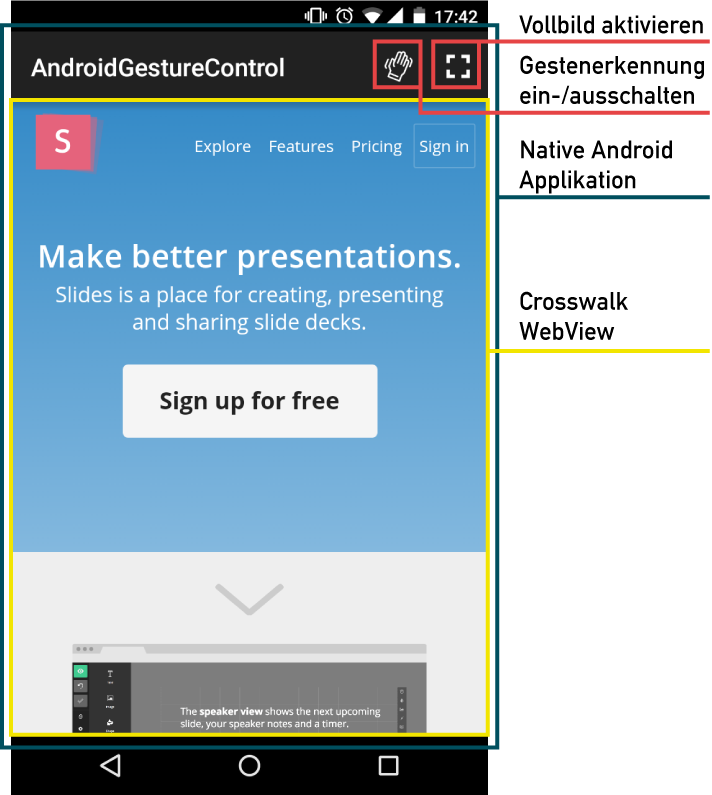
\includegraphics[width=1\linewidth]{screenshot-ui-beschriftet.png}}
\end{minipage}
\caption{Screenshot App mit Slides.com-Startseite.}
\label{fig:ui}
\end{figure}

\subsection{Slides.com}
Das bereits erwähnte Reveal.js-Framework ist unter der freien MIT Lizenz verfügbar. Mit \url{slides.com} hat der Entwickler Hakim El Hattab eine Freemium-Plattform bereitgestellt, die eine Web-App für die Erstellung der Decks/Präsentationen im Reveal.js Style und Format realisiert. Durch den Einsatz des Services wird ein bewährtes Tool zur Erstellung und Verwaltung der Decks eingesetzt und der Nutzer kann sich sowohl in der App als auch am Computer in sein Slides.com-Konto einloggen.


\subsection{Native Android-App mit WebView}
Um Slides.com und die Gestenerkennung per JavaScript in einer nativen Android-App kombinieren zu können, wird die Web-App in einem WebView aufgerufen und das modifizierte gesture.js-Skript injiziert. Es handelt sich somit um eine \textit{WebView Application} \cite{webview14}. Da der von Android  bereitgestellte WebView stark eingeschränkt ist und keinen direkten Zugriff auf die Kamera des Geräts zulässt, wird der alternative WebView des \textit{Crosswalk Project} \footnote{\url{https://crosswalk-project.org}} eingesetzt. Dieser ist ein In-App Browser mit vollem Funktionsumfang des aktuellsten Chromium-Browsers mit der Rendering-Engine \textit{Blink} \footnote{\url{http://www.chromium.org/blink}}. Durch den Crosswalk-WebView ist das direkte Ansprechen der Kamera mittels WebRTC API möglich.

\begin{figure}[htb]
\begin{minipage}[b]{1.0\linewidth}
  \centering
\centerline{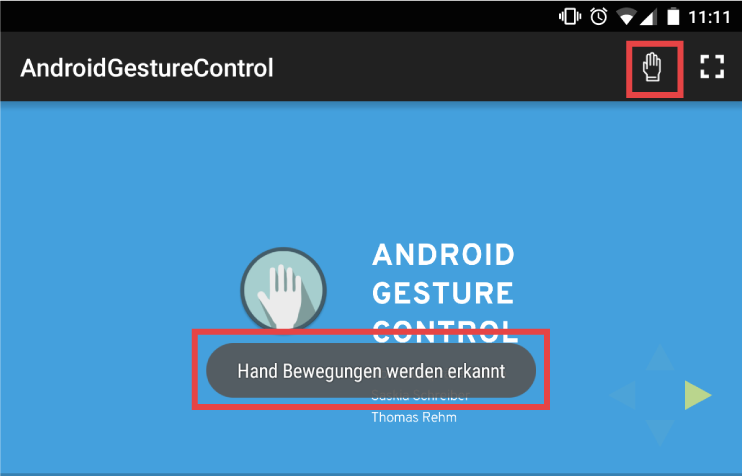
\includegraphics[width=1\linewidth]{screenshot-ui-toast-quer.png}}
\end{minipage}
\caption{Screenshot App im Querformat mit aktivierter Gestenerkennung.}
\label{fig:toast}
\end{figure}

\subsection{Benutzerinteraktion}
Wichtig für ein intuitives Erlebnis ist auch die Bedienung der App, die mit wenigen Buttons ihre Funktionalität bereitstellt.
So befinden sich neben dem WebView mit den Bedienelementen der Web-App noch je ein Button für die Aktivierung des Vollbild-Modus und für das Ein- und Ausschalten der Gestenerkennung (siehe Fig. \ref{fig:ui}).
Wird die Gestensteuerung vom Nutzer aktiviert, ändert sich das Piktogramm und dem Nutzer wird in einer kurzen Nachricht mitgeteilt, dass jetzt die Bewegungen erkannt werden (siehe Fig. \ref{fig:toast}).

\subsection{Präsentieren mit AndroidGestureControl}
\label{ref:present}
Die eigentliche Ausgabe und Präsentation des Bildes erfolgt mittels Bildschirmübertragung des Android-Bildschirms an einen Beamer oder Fernseher. Die Übertragung kann per Kabel via \textit{MHL (Mobile High-Definition Link)}\footnote{\url{http://mhlconsortium.org/consumer.aspx}} direkt an den HDMI-Anschluss des Beamers/TVs oder per WLAN an einen passenden Empfänger mit HDMI-Anschluss übertragen werden. Dabei wird ein HDMI-Stick eingesetzt, der ein passendes Übertragungsprotokoll wie \textit{Google Cast} \footnote{\url{https://developers.google.com/cast/}}, \textit{Miracast} \cite{ijitr555} oder \textit{Apple AirPlay}\footnote{\url{https://support.apple.com/de-de/HT204289}} unterstützt. Einige SmartTVs unterstützen die genannten Protokolle bereits und benötigen keinen zusätzlichen Stick. Die drahtlose Übertragung des Bildschirms bietet dem Präsentierenden eine höhere Freiheit als die kabelgebundene Lösung. Die genutzten Geräte müssen lediglich über das gleiche drahtlose Netzwerk verbunden sein. Teilweise benötigen die Geräte einen Internetzugang, um die Daten zu übertragen; in jedem Fall muss die Präsentation zuvor per Internet aufgerufen werden.

\section{Zusammenfassung und Bewertung der Ergebnisse}
Im Rahmen dieser Arbeit wurden verschiedene Technologien kombiniert, um das gesetzte Ziel zu erreichen: Gestensteuerung über Kamerainformationen auf der einen und Screen Mirroring auf der anderen Seite.\\
Gestensteuerung auf Mobilgeräten einzusetzen ist offensichtlich kein Problem mehr und dank der Nutzung von Webtechnologien auch nicht auf Android beschränkt. Die Rechenleistung der Geräte reicht dafür aus, auch wenn die Genauigkeit der im Prototyp eingesetzten Algorithmen noch feiner sein könnte. Da die Umrechnung der Bilddaten in Gesten jedoch nicht das Kernthema darstellt, ist das Ziel aus Sicht der Autoren dennoch voll erreicht worden.\\ Weitere Themen ergeben sich natürlich: Device-übergreifende Performancetests könnten beispielsweise aufzeigen, wo noch Spielraum für mehr Datentransfer und somit genauere Gestenerkennung ist.\\
Bei der Auswahl des Protokolles zur Verbindung der Geräte wurden sowohl Google Cast als auch Miracast über Set-Top-Boxen getestet. Beide Varianten funktionieren, haben aber Einschränkungen in Handhabung und Stabilität. Eine direkte Nutzung der Protokolle durch SmartTVs ist damit ein wichtiges Kriterium für die Alltagstauglichkeit des vorgestellten Systems. Das wiederum setzt voraus, dass in den Präsentationsräumen überhaupt ein SmartTV zur Verfügung steht. Entsprechende Statistiken \cite{statistatv} zeigen, dass diese zumindest in privaten Haushalten immer mehr an Bedeutung gewinnen.
\newpage


% References should be produced using the bibtex program from suitable
% BiBTeX files (here: strings, refs, manuals). The IEEEbib.bst bibliography
% style file from IEEE produces unsorted bibliography list.
% -------------------------------------------------------------------------
%\bibliographystyle{IEEEbib}

\bibliographystyle{IEEEtran}
%\vfill
%\pagebreak
\bibliography{refs}

\end{document}
